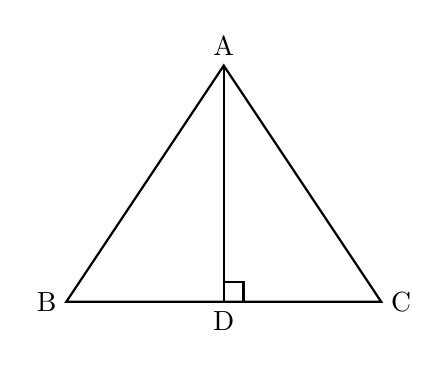
\begin{tikzpicture}[scale=1]
  % Define coordinates to match the visual proportions of the image
  \coordinate (A) at (0, 3);    % Top vertex
  \coordinate (B) at (-2, 0);   % Bottom left
  \coordinate (C) at (2, 0);    % Bottom right
  \coordinate (D) at (0, 0);    % Intersection on base

  % Draw the main triangle ABC
  \draw[thick] (A) -- (B) -- (C) -- cycle;

  % Draw the altitude AD (vertical line)
  \draw[thick] (A) -- (D);

  % Draw the right-angle marker at D (0.25 unit square)
  \draw[thick] (0, 0.25) -- (0.25, 0.25) -- (0.25, 0);

  % Add labels exactly as positioned in the image
  \node[above] at (A) {A};
  \node[left] at (B) {B};
  \node[right] at (C) {C};
  \node[below] at (D) {D};

\end{tikzpicture}